\documentclass[12pt,a4paper]{extarticle}
\usepackage{ascmac, amsmath,amssymb, url, pifont, jumoline, wrapfig}
%\usepackage{bm}
\usepackage[at]{easylist}
\usepackage[dvipdfmx]{graphicx, xcolor} % 枠組み
\usepackage{tikz}
\usepackage[framemethod=tikz]{mdframed}
\usepackage[top=10truemm,bottom=10truemm,left=20truemm,right=20truemm]{geometry}
\renewcommand{\baselinestretch}{1.5}
\renewcommand{\figurename}{図}
\pagestyle{empty}
\global\mdfdefinestyle{exampledefault}{%
	middlelinewidth=1pt,%
	leftmargin=1cm,rightmargin=1cm}
\makeatletter 
\def\section{\@startsection {section}{1}{\z@}{-3.5ex plus -1ex minus -.2ex}{2.3 ex plus .2ex}{\large\bf}} % change section style
\def\subsection{\@startsection {subsection}{1}{\z@}{-3.5ex plus -1ex minus -.2ex}{2.3 ex plus .2ex}{\normalsize\bf}}
\makeatother

\newcommand{\point}[1]
{\textbf{\textcolor{magenta}{#1}}}
\newcommand{\obs}[1]
{\textbf{\textcolor{violet}{#1}}}
\newcommand{\rec}[1]
{\textbf{\textcolor{orange}{#1}}}
%#######*****#######*****#######*****#######***
\begin{document} 

\noindent\textbf{\Large{函南毎木調査マニュアル} \small{(140820 瓜生作成) ver.1.0}}\\

毎木調査は過去データの蓄積を利用しており、今回のデータも次回以降の調査に活用される。{\large{測定者、記録者それぞれが責任を持ち、役割を果たすように努めること。}}

\section*{作業内容}

プロット内に生育する木本植物を対象に、\textbf{胸高直径5cm 以上の個体・幹}について計測を実施する。基本的に\point{測定者}2名と\point{記録者}1名での3名一組で行う。2組で調査を行う場合には各組で1列を担当する。

\subsection*{プロット設計}

函南原生林内の600mから800mまでの範囲に、100m間隔で3つのプロットが設置されている。\textbf{各プロットの面積は600m 2.0ha、700m 1.1ha、800m 1.1ha}である(図1)。すべての\textbf{プロットは10m $\times$ 10mのメッシュに分割}されており、アルファベットと数字からなるメッシュ番号が与えられている(e.g. \textbf{A14})。

\begin{figure}[hb]
\centering
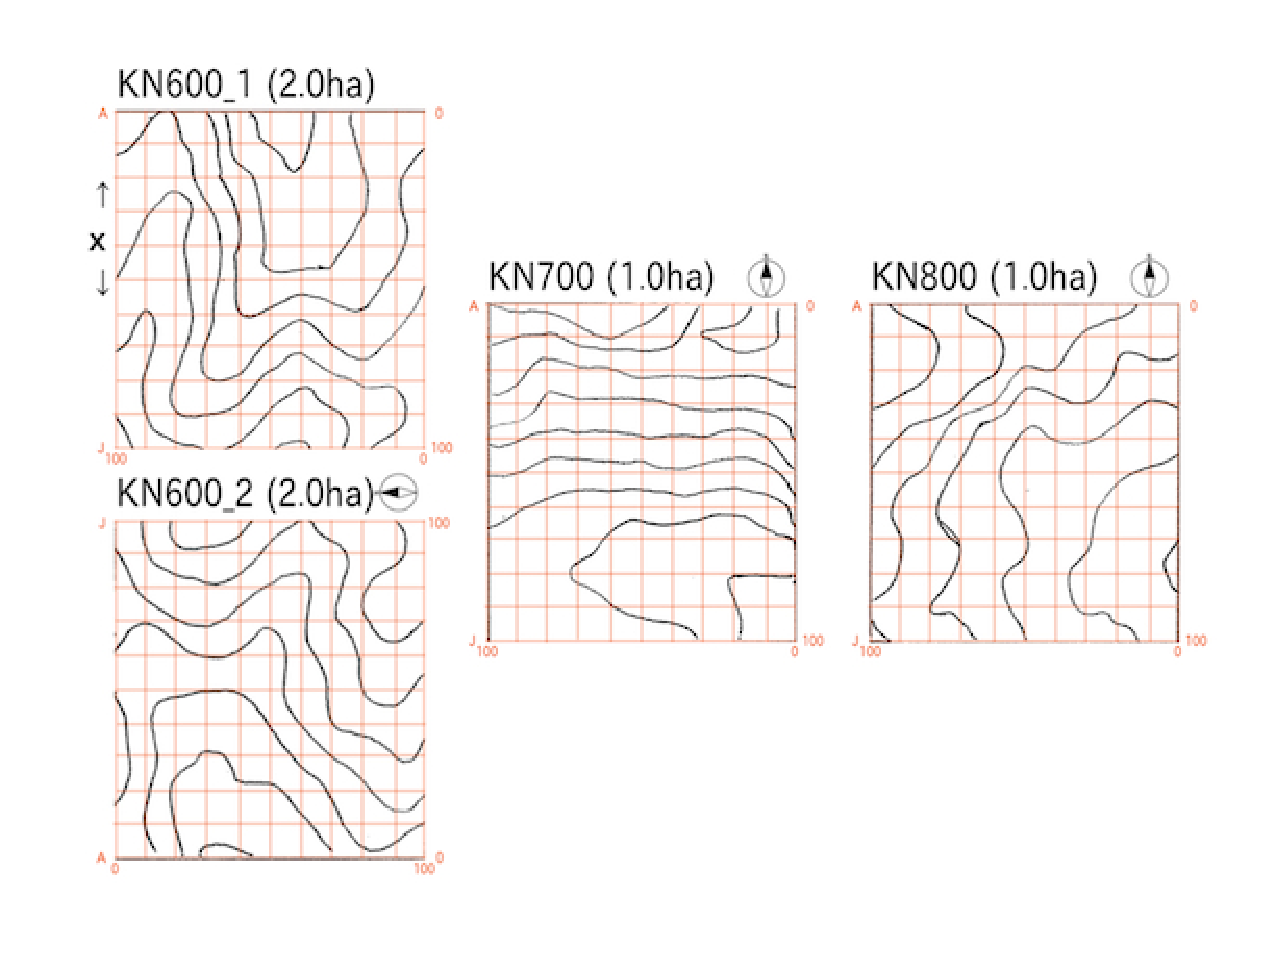
\includegraphics[scale=0.6]{../Images/plot_design.eps}
\caption{函南原生林3プロットのデザイン}
\end{figure}

\newpage
\subsection*{大まかな手順}

\begin{easylist}[enumerate]
@ メッシュ内に生育する個体を探す
@ 調査する個体の\point{胸高周囲長}およびその他の項目を測定・記録する
@ \point{新規個体}にタグを取り付け、種同定をした後に胸高周囲長を測定する
@@ 過去の調査で記録されていない胸高直径5cm以上の個体・幹を新規として扱う
\end{easylist}

\subsection*{計測項目}

各個体・幹について次の項目を測定し、調査シート(図2)に記録する。この他、記録者はメッシュ内での個体位置、調査中に気がついたことなどをデータシートに記載する。また、測定者は測定状況などを測定値とともに伝えるようにする。

\begin{easylist}[enumerate]
@ \textbf{胸高周囲長}(\point{GBH$_{14}$}): 地上高1.3m... おおよそ自分の胸の高さでの樹木の幹周囲(cm; 有効数字3桁)
@@ 過去のサイズと比較し、もし値が小さくなっている場合には再計測を行う
@@ 同一個体で複数の幹を持つ場合、「\textbf{個体●●の萌芽}」など、同一個体のものであることがわかるようにする
@ \textbf{萌芽幹の本数}(\point{Spr$_{14}$}): 地際30cm以下から発生している萌芽の本数
@ \Midline{光環境の評価}(\point{CPI$_{14}$}): 樹冠の位置により4段階で区分。データシート参照
@ \textbf{生死の判定}(\point{LD$_{14}$}): 生存なら0(または無記入)、\textbf{死亡ならば1}とする
@@ 死亡要因は\point{Note}欄に記録する。死亡要因としては枯死、幹折れ、根返りがある
\end{easylist}

\begin{figure}[hb]
\centering
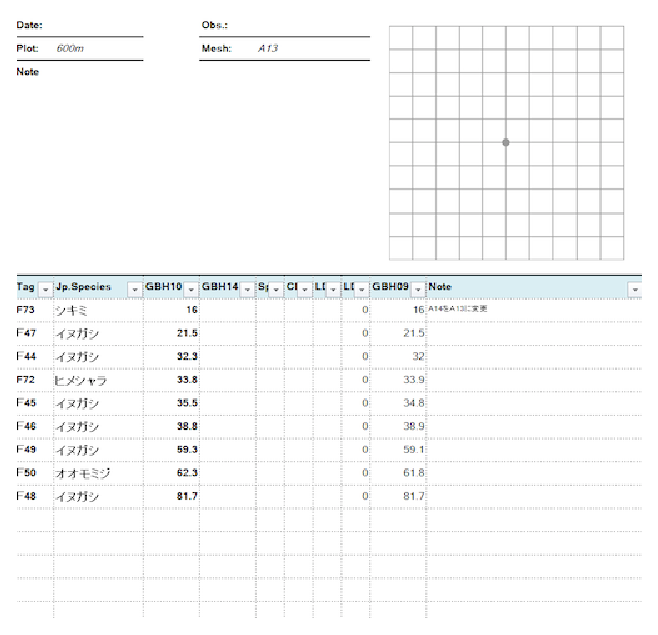
\includegraphics[scale=0.6]{../Images/datasheet-sample.eps}
\caption{調査シートの見本}
\end{figure}

\newpage
\begin{mdframed}[style=exampledefault,roundcorner=5]\small{
\subsubsection*{胸高周囲長の測り方}

\begin{wrapfigure}{r}{50mm}
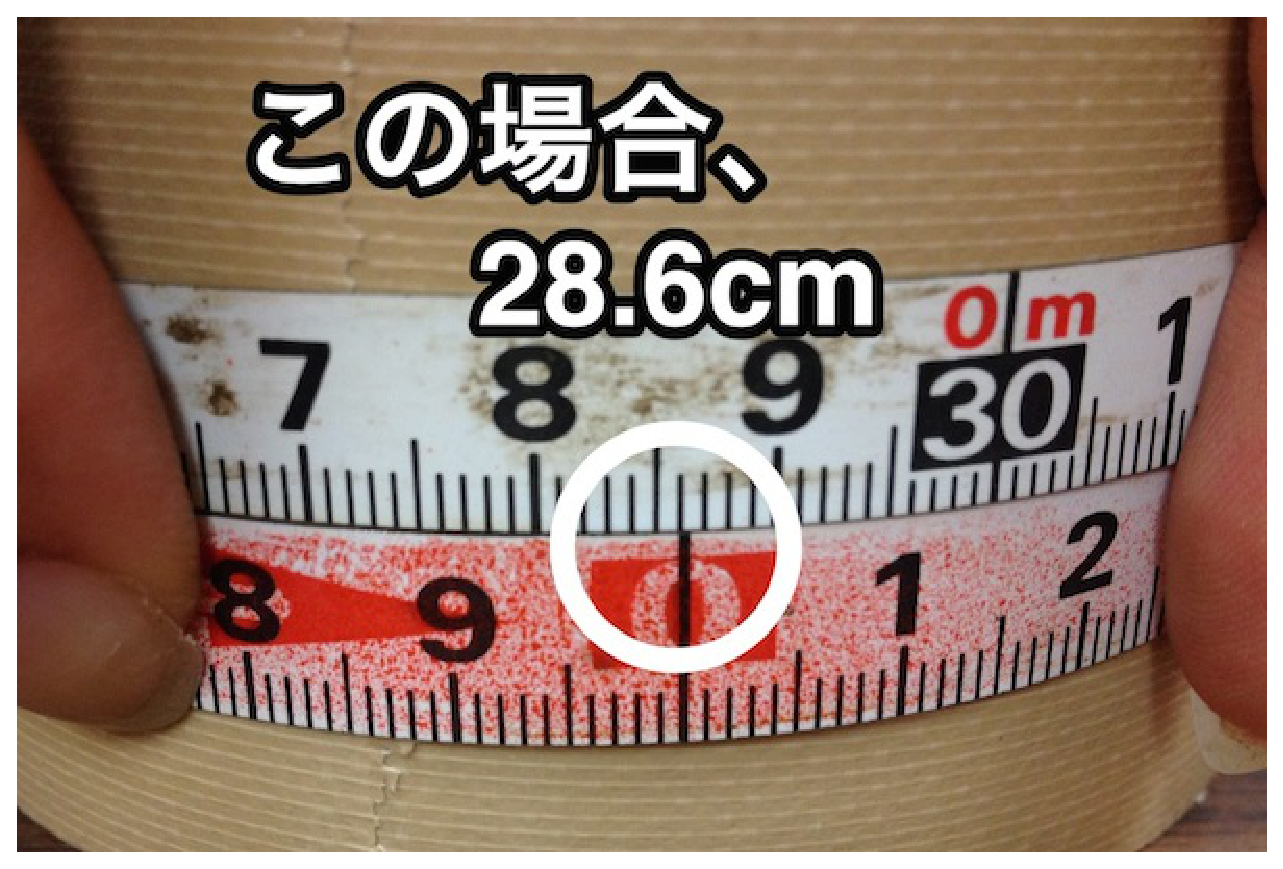
\includegraphics[scale=0.24]{../Images/measure.eps}
\end{wrapfigure}


タグがついている幹につけられた赤いスプレー跡に沿って、スチールメジャーを巻き付ける。この時、メジャーが斜めになっていたり、途中で裏返っていると測定誤差が生じるため、\textbf{まっすぐに裏返らないよう}、確認しながら幹に巻きつけること。巻き付けたら、メジャーを左右にしごき、目盛りが最小になるところで落ち着かせる。その後、強くメジャーを締め、周囲長の値を読む。このとき、\textbf{メジャーの先側となる0cmが下側}、伸ばした側が上に来るようにする(※使用するメジャーは先端から数cm先に0cmの基準があるのでそこに合わせる)。

}\end{mdframed}

\begin{mdframed}[style=exampledefault,roundcorner=5]\small{
\subsubsection*{新規個体の測定・記録方法}

新規個体は\textbf{次回の調査以降でも使う}ものなので、間違いがないよう十分気をつける。 新規個体を発見したら、測定位置を決める。基本的には自分の胸の高さ(およそ地上1.3m)を測定位置とするが、障害物(コブ、ツル、他の幹など)がある場合には前後20cmの範囲を測定位置とする。測定位置を決めたら、そこから10cm上に金槌でタグ・釘を取り付ける(深さ1cm程度)。タグをつけたら種を同定する。同定が不安な場合、近くにいる人と相談して種名を記録し、備考欄にその旨を書く。胸高周囲長を測り、メジャーを強く締めた状態のまま、メジャーの上から幹に沿ってスプレーでマークする。

}\end{mdframed}

\subsubsection*{その他}

\begin{easylist}[itemize]
@ 調査をした個体には\textbf{チョーク}で印(サイズやタグ番号)をつけておくと測定の重複を防ぐことができる
@ データシートに記録できない個体・幹は野帳に記録しておく(\point{メッシュ番号、タグ番号を必ず書くこと})
@ ササの多いメッシュでは個体を探すのが大変...記録者が指示してあげると良い
@ どうしても対象個体が見つからない場合は\textbf{消失}として欠測であることを記録
@@ 倒木してタグが隠れている可能性もあるので倒れた幹なども確認
@ \textbf{新規個体の基準となる5cm}の大きさを把握しておくと良い。

\rule{5.2cm}{1.4pt}←これが5cmの長さ(親指の長さ+$\alpha$くらい)。

@ 斜面では原則として山側に立ち、タグを取り付ける
\end{easylist}

\end{document} 